\notechapter{N-20261015}{Twelvefold Counting: What Labels Remember}

Suppose four people must be placed into three nonempty groups. With group names, there are \(36\) assignments; without group names, there are \(6\) partitions of the four people; if the people are also indistinguishable, the only possible pattern is \(2+1+1\). All three answers are correct. What changed was the amount of information we agreed to remember.

The \emph{twelvefold way} arranges such questions into a single scheme. More unexpectedly, its entries lead to group actions, Stirling numbers, finite differences and two rather different sorts of generating functions. We will try to recover the formulas from the objects they count, so that the table can eventually be remembered without memorizing its entries.\footnote{The classical table and its precise mapping formulation appear in \href{https://dlmf.nist.gov/26.17}{NIST Digital Library of Mathematical Functions, \S26.17}, following Richard Stanley's \emph{Enumerative Combinatorics}, Vol.~1.}

\section{A distribution is a function}

Take \(n\) balls and \(k\) boxes, initially with both sorts of labels. Every distribution is a function
\[
 f:[n]\longrightarrow[k],\qquad
 i\longmapsto\text{the box containing ball }i.
\]
It is worth asking which extra properties of \(f\) can be imposed. With no restriction, there are \(k^n\) functions. If no two balls may share a box, \(f\) must be injective; if every box must be used, \(f\) must be surjective.

For \(n=4\), \(k=3\), the distribution
\[
 A,B\longmapsto1,\qquad C\longmapsto2,\qquad D\longmapsto3
\]
has a particularly useful fourfold description. If we remove the names from the balls while retaining the names of the boxes, we remember only the \emph{occupancy vector} \((2,1,1)\). If we keep the ball names but remove the box names, we remember which balls were together:
\[
 \bigl\{\{A,B\},\{C\},\{D\}\bigr\}.
\]
Finally, with neither sort of name, we remember just the multiset of positive occupancies, customarily written as an integer partition \(4=2+1+1\).

\begin{figure}[htbp]
\centering
\begin{tikzpicture}[>=Stealth,
 every node/.style={font=\small},
 box/.style={draw=purple!55!black,rounded corners=3pt,fill=purple!3,
             inner xsep=8pt,inner ysep=7pt,align=center}]
 \node[box] (f) at (-3.1,1.45) {\(A,B\mapsto1;\ C\mapsto2;\ D\mapsto3\)};
 \node[box] (o) at (3.1,1.45) {\((2,1,1)\)};
 \node[box] (s) at (-3.1,-1.35) {\(\{\{A,B\},\{C\},\{D\}\}\)};
 \node[box] (p) at (3.1,-1.35) {\(2+1+1\)};
 \draw[->,thick] (f)--node[above,fill=white,inner sep=2pt,font=\scriptsize]
    {forget ball names} (o);
 \draw[->,thick] (f)--node[left,fill=white,inner sep=2pt,font=\scriptsize]
    {forget box names} (s);
 \draw[->,thick] (o)--node[right,fill=white,inner sep=2pt,font=\scriptsize]
    {forget box names} (p);
 \draw[->,thick] (s)--node[below,fill=white,inner sep=2pt,font=\scriptsize]
    {forget ball names} (p);
\end{tikzpicture}
\caption{Four descriptions of one assignment. The arrows discard information; reversing them requires choices and usually does not give a unique answer.}
\end{figure}

One subtlety will matter throughout: an unused box still exists. In the occupancy vector it appears as a zero; in a set partition or an integer partition it disappears. Thus \(k\) boxes without names permit \emph{at most} \(k\) nonempty blocks, unless we insist that all boxes are occupied.

\section{The twelve entries}

Let \(S(n,j)\) denote the number of ways to partition an \(n\)-element labelled set into exactly \(j\) nonempty, unordered blocks. Let \(p_{\le k}(n)\) and \(p_{=k}(n)\) count integer partitions of \(n\) into at most \(k\), respectively exactly \(k\), positive parts. Put
\[
 (k)_{\underline n}=k(k-1)\cdots(k-n+1),
 \qquad [P]=\begin{cases}1,&P\text{ is true},\\0,&P\text{ is false}.\end{cases}
\]
Here \(n,k\ge1\), and an impossible configuration has count zero.

\begin{table}[htbp]
 \centering
 \small
 \setlength{\tabcolsep}{5pt}
 \renewcommand{\arraystretch}{1.75}
 \begin{tabular}{@{}lccc@{}}
 \toprule
 Labels retained & Unrestricted & Injective & Surjective\\
 \midrule
 Balls and boxes &
 \(k^n\) & \((k)_{\underline n}\) & \(k!S(n,k)\)\\
 Boxes only &
 \(\binom{n+k-1}{k-1}\) & \(\binom{k}{n}\) & \(\binom{n-1}{k-1}\)\\
 Balls only &
 \(\sum_{j=1}^k S(n,j)\) & \([n\le k]\) & \(S(n,k)\)\\
 Neither &
 \(p_{\le k}(n)\) & \([n\le k]\) & \(p_{=k}(n)\)\\
 \bottomrule
 \end{tabular}
 \caption{The twelvefold way for \(n,k\ge1\). Empty boxes may occur in the unrestricted and injective columns.}
\end{table}

It is enough to know four kinds of objects---functions, occupancy vectors, set partitions, integer partitions---and three restrictions on the fibers of a function. We now derive the rows, partly to check the table and partly to understand where their formulas come from.

\section{Reconstructing the table}

With both sorts of labels, unrestricted functions give \(k^n\); injections give \((k)_{\underline n}\). For surjections, first partition the \(n\) balls into \(k\) nonempty blocks, then match those blocks bijectively with the \(k\) named boxes. This gives \(k!S(n,k)\). The factor \(k!\) is justified because every box is used: the blocks really can be assigned \(k!\) different lists of names.

If only boxes are labelled, write \(a_i\) for the number of balls in box \(i\). An unrestricted arrangement is a solution
\[
 a_1+\cdots+a_k=n,\qquad a_i\ge0.
\]
Arrange \(n\) stars in a row and insert \(k-1\) separators among the \(n+k-1\) available positions. Consecutive separators indicate empty boxes, and we obtain
\[
 \#\{(a_i)\in\mathbb Z_{\ge0}^k:\sum a_i=n\}
 =\binom{n+k-1}{k-1}.
\]
For injections, the occupancies belong to \(\{0,1\}\), so we choose \(n\) of the \(k\) boxes. For surjections, \(a_i\ge1\); setting \(b_i=a_i-1\) gives \(\binom{n-1}{k-1}\). The difference between weak and positive compositions is just a shift of one in every coordinate.

If only balls are labelled, the nonempty fibers \(f^{-1}(i)\) form an unordered set partition. In the unrestricted case it may have \(1,2,\ldots,k\) blocks, giving \(\sum_{j=1}^kS(n,j)\). Surjectivity fixes the number of blocks at \(k\). Injectivity makes every block a singleton, leaving exactly one partition when \(k\ge n\).

Finally, if neither sort of label remains, the only information is a nonincreasing sequence of positive occupancies
\[
 \lambda_1\ge\lambda_2\ge\cdots\ge\lambda_\ell\ge1,
 \qquad \lambda_1+\cdots+\lambda_\ell=n.
\]
An unrestricted arrangement has \(\ell\le k\); a surjection has \(\ell=k\); an injection has only parts equal to \(1\). These are precisely the last three entries.

\begin{remark}
A useful memory test is to redraw the table from a blank sheet using the words
\[
 \text{function},\quad
 \text{weak composition},\quad
 \text{set partition},\quad
 \text{integer partition}.
\]
The middle column asks that every fiber have size at most one; the last column requires every fiber to be nonempty. No separate list of twelve formulas is needed.
\end{remark}

\section{Forgetting names}

Why is removing a label an operation that can be studied mathematically? Let
\(\mathcal F=\{f:[n]\to[k]\}\). Permutations \(\sigma\in S_n\) and \(\tau\in S_k\) act on a function by
\[
 (\sigma,\tau)\cdot f=\tau\circ f\circ\sigma^{-1}.
\]
Relabelling the balls changes which input carries a given identity; relabelling the boxes changes the names of the outputs. The injective and surjective subsets are invariant under these actions.

Two functions lie in the same \(S_n\)-orbit exactly when they have the same occupancy vector \((a_1,\ldots,a_k)\). Their fibers have the same labelled sizes, and a bijection can be chosen between corresponding fibers. Two functions lie in the same \(S_k\)-orbit exactly when they have the same partition of the labelled domain into nonempty fibers. Allowing both actions leaves only the integer partition of the nonzero occupancies.

Thus the first three lines of our diagram can be written as quotients:
\[
 \mathcal F,\qquad \mathcal F/S_n,\qquad
 \mathcal F/S_k,\qquad
 \mathcal F/(S_n\times S_k).
\]
It is tempting to divide \(k^n\) by \(k!\) after forgetting the names of the boxes. Take one ball and three boxes: there are three labelled assignments, but just one unlabelled assignment. Dividing by \(3!=6\) would give \(1/2\). The two empty boxes may be swapped without changing the assignment, so this assignment has fewer than six distinct relabellings.

For a group \(G\) acting on a set \(X\), write \(Gx\) for the orbit of \(x\) and \(G_x\) for its stabilizer. Counting the group elements mapping \(x\) to the same point gives
\[
 |Gx|=\frac{|G|}{|G_x|}.
\]
Orbits need not have equal sizes. A particularly useful way to count them is the following.

\begin{theorem}[Burnside's lemma]
For a finite group \(G\) acting on a finite set \(X\),
\[
 \boxed{|X/G|=\frac1{|G|}\sum_{g\in G}|\operatorname{Fix}(g)|.}
\]
\end{theorem}
\begin{proof}
Count pairs \((g,x)\) satisfying \(gx=x\), once by the group element and once by the point:
\[
 \sum_{g\in G}|\operatorname{Fix}(g)|
 =\sum_{x\in X}|G_x|.
\]
Within each orbit, every stabilizer has cardinality \(|G|/|Gx|\); summing \(|G_x|\) over that orbit gives \(|G|\). Divide by \(|G|\).
\end{proof}

For example, color six beads black or white on a circular necklace; rotations count as the same pattern. A rotation by \(r\) positions breaks the bead positions into \(\gcd(6,r)\) cycles. A coloring survives the rotation precisely when every such cycle is monochromatic. Its fixed-point count is \(2^{\gcd(6,r)}\). Hence
\[
 \#\text{necklaces}
 =\frac{2^6+2^1+2^2+2^3+2^2+2^1}{6}
 =14.
\]
The acting group here is the cyclic group \(C_6\), rather than the full symmetric group \(S_6\). This is the beginning of P\'olya counting: specify which symmetries are allowed, then count colorings constant on their cycles. It is also why a geometrically arranged collection of boxes often requires a different counting theory from the twelvefold table.

\section{Stirling numbers appear when a new ball arrives}

Return to \(S(n,k)\). Insert the element \(n\) into a partition of \([n]\) with \(k\) blocks. Either \(n\) forms a singleton block, leaving a partition of \(n-1\) elements into \(k-1\) blocks, or it joins one of the \(k\) existing blocks of a partition of \(n-1\) elements into \(k\) blocks. Therefore
\[
 \boxed{S(n,k)=S(n-1,k-1)+kS(n-1,k).}
\]
With \(S(0,0)=1\), \(S(n,0)=0\) for \(n>0\), this gives
\[
\begin{array}{c|rrrrr}
 n\backslash k &0&1&2&3&4\\ \hline
 0&1&&&&\\
 1&0&1&&&\\
 2&0&1&1&&\\
 3&0&1&3&1&\\
 4&0&1&7&6&1
\end{array}
\]
In particular \(S(4,3)=6\), explaining the initial group problem: labelling the three nonempty groups gives \(3!\cdot6=36\) assignments.

There is another formula, useful when \(n\) is large and \(k\) is fixed. A function \([n]\to[k]\) fails to be surjective when at least one box is missed. Inclusion--exclusion over the missing boxes gives
\[
 \boxed{k!S(n,k)=\sum_{j=0}^k(-1)^j\binom{k}{j}(k-j)^n.}
\]
For \(n=4,k=3\), the right side is \(3^4-3\cdot2^4+3=36\). The recurrence and the alternating sum compute the same quantity through different decompositions: one inserts a new element, the other excludes forbidden images.

\section{From counting to polynomials}

Fix an integer \(m\ge0\). There are \(m^n\) functions from \([n]\) to \([m]\). Count these functions by the number \(j\) of distinct values they actually use. Their fibers form a partition into \(j\) blocks, and their \(j\) distinct images can be assigned to these blocks in \((m)_{\underline j}\) ways. Therefore
\[
 m^n=\sum_{j=0}^nS(n,j)(m)_{\underline j}.
\]
Both sides are polynomials in \(m\). Since they agree at every nonnegative integer, they agree for an indeterminate \(x\):
\[
 \boxed{x^n=\sum_{j=0}^nS(n,j)(x)_{\underline j}.}
\]
For example,
\[
 x^3=(x)_{\underline3}+3(x)_{\underline2}+(x)_{\underline1}
\]
and
\[
 x^4=(x)_{\underline4}+6(x)_{\underline3}
             +7(x)_{\underline2}+(x)_{\underline1}.
\]

This has a second interpretation. The usual monomials \(1,x,x^2,\ldots\) and the falling factorials
\[
 1,\quad x,\quad x(x-1),\quad x(x-1)(x-2),\ldots
\]
are two bases of the polynomial ring. The Stirling numbers of the second kind are the coefficients for changing from the first basis to the second. Reversing the change of basis defines the signed Stirling numbers of the first kind \(s(n,j)\):
\[
 (x)_{\underline n}=\sum_{j=0}^ns(n,j)x^j.
\]
For instance, \((x)_{\underline3}=x^3-3x^2+2x\). The two triangular arrays are inverse matrices. The reason is algebraic and concrete: each is a change of basis, and changing back recovers the original polynomial.

\section{The discrete derivative}

Define the forward difference
\[
 \Delta f(x)=f(x+1)-f(x).
\]
Ordinary differentiation is particularly simple on powers:
\(Dx^j=jx^{j-1}\). For finite differences, falling factorials play the same role:
\[
 \boxed{\Delta (x)_{\underline j}=j(x)_{\underline{j-1}}.}
\]
Indeed, using \((x)_{\underline j}=j!\binom{x}{j}\), this follows from Pascal's identity
\[
 \binom{x+1}{j}-\binom{x}{j}=\binom{x}{j-1},
\]
which is a polynomial identity in \(x\).

Repeated differences now provide a discrete version of Taylor's formula. If \(f\) is a polynomial of degree at most \(d\), then
\[
 \boxed{f(x)=\sum_{j=0}^d(\Delta^jf)(0)\binom{x}{j}.}
\]
To see this, expand \(f=\sum_jc_j\binom{x}{j}\) in the binomial basis. Successive differences satisfy \(\Delta\binom{x}{j}=\binom{x}{j-1}\); evaluating \(\Delta^rf\) at \(x=0\) leaves precisely \(c_r\).

Apply the formula to \(f(x)=x^n\), and compare with the Stirling expansion. We obtain the striking identity
\[
 \boxed{S(n,j)=\frac{(\Delta^j x^n)|_{x=0}}{j!}.}
\]
As \(\Delta^j f(0)=\sum_{i=0}^j(-1)^{j-i}\binom ji f(i)\), this is exactly
\[
 S(n,j)=\frac1{j!}
 \sum_{i=0}^j(-1)^{j-i}\binom ji i^n.
\]
The inclusion--exclusion formula for surjections has reappeared as the coefficient formula for a discrete derivative.

\begin{example}
Let \(f(x)=x^3\). Its successive values at \(0,1,2,3\) are \(0,1,8,27\). The difference rows begin with \(1,6,6\), so
\[
 x^3=\binom{x}{1}+6\binom{x}{2}+6\binom{x}{3}.
\]
Dividing the coefficients by \(1!,2!,3!\) recovers \(S(3,1)=1\), \(S(3,2)=3\), \(S(3,3)=1\). The recurrence triangle, inclusion--exclusion and Newton interpolation are three views of the same coefficients.
\end{example}

There is even an operator identity. Write \(D=d/dx\). Since \(xD\) sends \(x^m\) to \(mx^m\), the polynomial identity already proved implies, on polynomials,
\[
 \boxed{(xD)^n=\sum_{j=0}^nS(n,j)x^jD^j.}
\]
For \(n=2\), this reads \((xD)^2=x^2D^2+xD\). The two sides agree on each monomial \(x^m\), hence on every polynomial. The same Stirling numbers that count ways of grouping balls therefore appear when we rearrange compositions of differentiation and multiplication by \(x\).

\section{A partition's geometry}

The final row of the twelvefold table deserves its own geometry. Consider
\[
 7=4+2+1.
\]
Its Ferrers diagram is a collection of left-justified unit squares with row lengths \(4,2,1\). Reflect the diagram across its main diagonal. Its column lengths are \(3,2,1,1\), so the transposed picture represents
\[
 7=3+2+1+1.
\]

\begin{figure}[htbp]
\centering
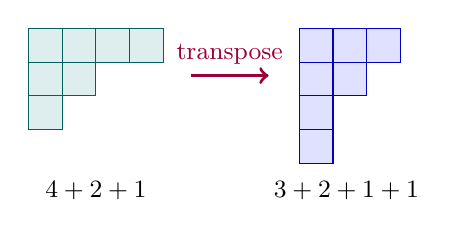
\begin{tikzpicture}[scale=.43]
 \foreach \x/\y in {0/0,1/0,2/0,3/0,0/-1,1/-1,0/-2}{
  \fill[teal!13] (\x,\y) rectangle ++(1,-1);
  \draw[teal!75!black,thin] (\x,\y) rectangle ++(1,-1);
 }
 \draw[->,very thick,purple!80!black] (4.8,-1.4)--(7.1,-1.4)
     node[midway,above,font=\small] {transpose};
 \foreach \x/\y in {8/0,9/0,10/0,8/-1,9/-1,8/-2,8/-3}{
  \fill[blue!12] (\x,\y) rectangle ++(1,-1);
  \draw[blue!75!black,thin] (\x,\y) rectangle ++(1,-1);
 }
 \node[font=\small] at (2,-4.8) {\(4+2+1\)};
 \node[font=\small] at (9.4,-4.8) {\(3+2+1+1\)};
\end{tikzpicture}
\caption{Conjugating an integer partition exchanges the number of rows and the largest row length.}
\end{figure}

The diagram proves a useful equinumerosity:
\[
 \boxed{p_{\le k}(n)=
 \#\{\lambda\vdash n:\text{every part of }\lambda\text{ is at most }k\}.}
\]
The left side limits the number of rows, while the right side limits their width. Diagram transposition is a bijection, even though there is no obvious term-by-term algebraic correspondence between the two descriptions.

For \(n=7,k=3\), the partition \(4+2+1\) has three parts and is admissible on the left, while its transpose \(3+2+1+1\) has largest part three and is admissible on the right. These are different partitions related by a canonical geometric operation.

\section{Products for parts}

Why do integer partitions naturally suggest products? For every permitted part size \(r\), we may use zero, one, two or more copies. Recording the total size by the exponent of \(x\), this independent choice contributes
\[
 1+x^r+x^{2r}+\cdots=\frac1{1-x^r}.
\]
Consequently, as an identity of formal power series,
\[
 \boxed{\sum_{n\ge0}p(n)x^n
       =\prod_{r\ge1}\frac1{1-x^r}.}
\]
If we permit only part sizes \(1,\ldots,k\), the product truncates:
\[
 \sum_{n\ge0}p_{\le k}(n)x^n
 =\prod_{r=1}^k\frac1{1-x^r},
\]
where the equality uses the conjugation bijection from the previous section.

To record \emph{exactly} how many parts we use, introduce a second variable:
\[
 \boxed{\sum_{n,\ell\ge0}p_{=\ell}(n)u^\ell x^n
  =\prod_{r\ge1}\frac1{1-u x^r}.}
\]
Here \(u\) marks the number of parts. For a fixed positive \(k\), removing one square from every row of a partition into \(k\) positive parts produces a partition of \(n-k\) into at most \(k\) parts. Hence
\[
 \sum_{n\ge k}p_{=k}(n)x^n
 =\frac{x^k}{(1-x)(1-x^2)\cdots(1-x^k)}.
\]
These formulas encode both restrictions appearing in the unlabelled--unlabelled row of the twelvefold table.

\section{Exponentials for blocks}

A set partition is built from \emph{labelled} elements. Let \(B_n=\sum_{k=0}^nS(n,k)\), the \(n\)-th Bell number. For a fixed \(k\), the exponential generating function for a nonempty labelled block is
\[
 e^x-1=\sum_{r\ge1}\frac{x^r}{r!}.
\]
If we arrange \(k\) nonempty blocks in a definite order, the labelled product construction gives \((e^x-1)^k\). Forgetting the order of the blocks divides by \(k!\), since every block is nonempty and therefore distinct as a set. We get
\[
 \boxed{\sum_{n\ge0}S(n,k)\frac{x^n}{n!}
 =\frac{(e^x-1)^k}{k!}.}
\]
Summing over all \(k\) gives the exponential formula
\[
 \boxed{\sum_{n\ge0}B_n\frac{x^n}{n!}
       =\exp(e^x-1).}
\]
For a quick consistency check, fix the block containing element \(n+1\) in a partition of \([n+1]\). Choose \(r\) of the other \(n\) elements to join it, and partition the remaining \(n-r\) elements in any way:
\[
 B_{n+1}=\sum_{r=0}^n\binom nr B_{n-r}.
\]
Differentiating \(B(x)=\exp(e^x-1)\) produces \(B'(x)=e^xB(x)\), and comparing coefficients reproduces the same recurrence.

The contrast with Euler's product is informative. For an integer partition, each numerical part size can be repeated independently, so we multiply geometric series. For a set partition, every block consumes a subset of a common pool of labelled elements; choosing how those labels are shared introduces binomial coefficients and factorial denominators. This is why exponential generating functions are adapted to labelled constructions and ordinary generating functions to the unrestricted multiplicities of integer parts.

The twelvefold table began with four ways of remembering the same distribution. It has now supplied two polynomial bases and two kinds of generating functions. There is a remaining question that the table alone cannot answer: if we select a labelled distribution uniformly at random and then forget its labels, are all the resulting unlabelled objects equally likely? The answer depends on the sizes of the orbits, and it leads to an entirely different side of combinatorics.
